\documentclass[pldi,amsmath,amssymb]{sigplanconf-pldi15}

\usepackage{graphics}
\usepackage[pdftex]{graphicx}% Include figure files
\usepackage{bm}
\usepackage{natbib} % necessary for bibtex
\usepackage[toc,page]{appendix}
\usepackage{pgffor}
\usepackage{minted}
\usepackage{syntax}
\usepackage{multicol}

% Suggested PLDI packages
\usepackage{SIunits}            % typset units correctly
\usepackage{courier}            % standard fixed width font
\usepackage[scaled]{helvet} % see www.ctan.org/get/macros/latex/required/psnfss/psnfss2e.pdf
\usepackage{url}                  % format URLs
\usepackage{listings}          % format code
\usepackage{enumitem}      % adjust spacing in enums
\usepackage[colorlinks=true,allcolors=blue,breaklinks,draft=false]{hyperref}   % hyperlinks, including DOIs and URLs in bibliography
\newcommand{\doi}[1]{doi:~\href{http://dx.doi.org/#1}{\Hurl{#1}}}   % print a hyperlinked DOI

% Grammar formatting
\setlength{\grammarparsep}{4pt plus 1pt minus 1pt}
\setlength{\grammarindent}{30em}

% minted haskell
\newmintinline[hsk]{haskell}{fontsize=\small}

\newcounter{quotecount}
\newcommand{\Question}[1]{\vspace{1cm}\addtocounter{quotecount}{1}%
     \parbox{10cm}{\em #1}\hspace*{2cm}(\arabic{quotecount})\\[1cm]}

\newcommand{\ignore}[1]{}

\begin{document}

\title{Using Probabilistic Programming Languages to
       Model Game Heuristics\\
  \null
  {\small \textnormal{
    Karl Cronburg\\
    \texttt{karl@cs.tufts.edu}\\
    \emph{Dept. of Computer Science, Tufts University, Medford MA 02155}\\
  }}
}

\maketitle
%\begin{abstract}
%\end{abstract}

% Introduction

\section{Introduction} \label{sec:intro}
A {\bf game-play heuristic} is a description of what a player should do to maximize their
utility in a game. Due to the probabilistic nature of many games, this description
can be formulated as a {\bf probabilistic model}. Repeated sampling from this model
gives the modeler a top-down view of what the heuristic does.
The modeler can then, given an inference engine, query the state of the game given
some observations about a state of the game at a different point in time.

It is apparent from this description that game-play heuristics fit
into the model-observe-query pattern used by existing Probabilistic Programming
Languages (PPLs).
In this work we present an argument favouring the use of PPLs
for describing game heuristics and reasoning about their performance.

%We now continue in Section \ref{sec:moq} with a discussion of how the probabilistic
%observe-query model of computation is applicable to certain questions game designers
%and players might ask of a
%game heuristic.
We now continue by studying a particular game with sufficiently
complicated probabilistic game mechanics, Dominion, discussed in Section
\ref{sec:dom}.
The complexity of Dominion and our attempts to model and make queries gives
us insight into the desired features of a PPL, and advantages and disadvantages
of existing PPLs. We discuss these insights in Section \ref{sec:meta-analysis}.
This is followed in Section \ref{sec:future:dominion} with a discussion of
Dominion-specific future work. We also touch on in Section \ref{sec:future:PPL}
the future of PPLs in relation to their applicability to the domain of
game heuristics.

%Our goal is to show that probabilistic inference is directly applicable to game
%heuristics. We argue that the questions a heuristic designer is interested in can be
%reformulated in terms of the model-observe-query pattern used by existing
%PPLs.

%\section{Goals} \label{sec:goals}
% goals of this work in relation to PPL design

%Existing probabilistic
%The goals of the work presented in the



% The kinds of probabilistic models and queries relevant to game heuristics

% Probabilistics models, observations, and queries
\section{Model-Observe-Query} \label{sec:moq}
% Talk about how, in general, game heuristics can be expressively
% described using probablistic models

\subsection{Example Game}

\subsection{Markov Chain Monte-Carlo} \label{sec:mcmc}
% talk about how we use rejection sampling when performing inference
% on probabilistic distributions, and why this is sufficient for
% our purposes >>>>v

% (it's because the points in the state-space which
% evaluate to true in the condition are diffuse and high overall density in the state-space.
% this will generally be true for standard deckbuilding games because
% the uniform-card-shuffling does a robust job of diffusing points which
% evaluate to true across the state space. the uniform shuffling is an inherently
% smooth transformation on the state space. similarly the conditionally true
% points in the state-space are dense because the conditional distributions
% we look at in this paper are not very restrictive - i.e. the percentage of
% conditionally false points in the state-space is very low, making rejection
% sampling successful because it's generally easy to find a conditionally true
% point in the state space regardless of the prior you sample from.

In the future we would like to further study instances in which rejection
sampling is insufficient due to high rejection rates. High rejection rates
in the case of deck building games like Dominion will most likely be the
result of inference questions involving very restrictive conditioning.
While it is possible that a high rejection rate can be the result of
a non-diffuse true distribution, this is not indicative of an interesting
deck of cards. For example you could design a card which turns
of shuffling in the game resulting in a pathologically non-diffuse 

%conditional distributions we are
% currently trying to sample from 



% Probabilistic modeling in Hakaru as applied to game heuristics

%\section{Implementation - Existing Languages}
% Hakaru + BLOG



% Case study - Dominion

% modeling Dominion in Hakaru, and what kinds of questions are interesting
% to ask the model
\section{Case Study: Dominion} \label{sec:dom}

Dominion is a game we are familiar with. This game is known as a turn-based
deckbuilding game, where a player \emph{builds} a good deck by choosing what
cards to buy on their turn. The probabilistic component of deckbuilding games
arises from shuffling decks of cards at certain points in the game. In particular
in Dominion the cards a player plays can affect both when cards get shuffled
and the composition of the deck being shuffled. As a result, game-play heuristics
for Dominion are inherently intertwined with the probabilistic game state.

\subsection{Game State}

\subsection{Heuristics} \label{sec:dom:heuristics}
We

\subsection{Greedy Results}
We present results for the greedy heuristic just described in
Section \ref{sec:dom:heuristics}. The simplest query one might wish to ask of
the greedy heuristic is:

\begin{quote} \label{quote:dominion-query}
Given that we buy card $X$ with probability $p0$ and card $Y$ with
probability $(1 - p0)$, what is the distribution over the length of
the game?
\end{quote}

In this query, we have model parameters of:

\begin{itemize}
\item $X$  \mintinline{haskell}{:: Card}
\item $Y$  \mintinline{haskell}{:: Card}
\item $p0$ \mintinline{haskell}{:: Probability}
\end{itemize}

\begin{figure}
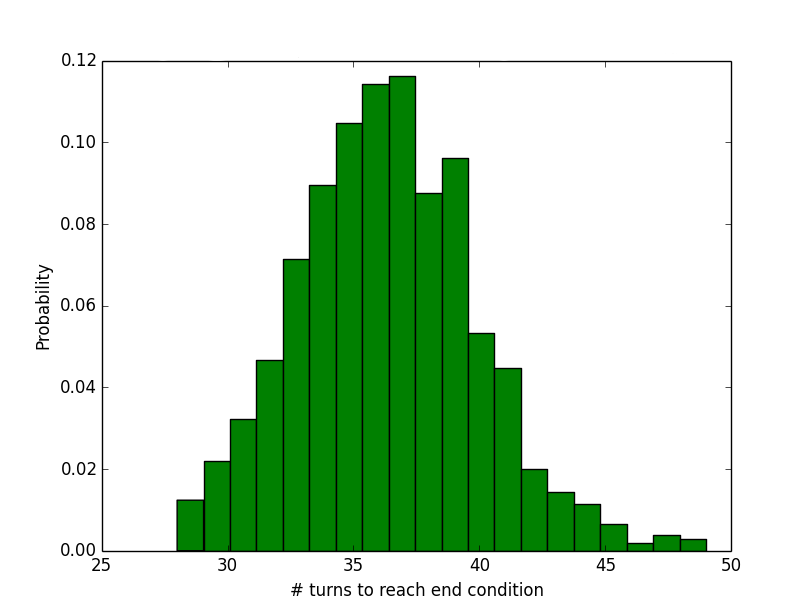
\includegraphics[width=.95\columnwidth]{../pres/village-chancellor-turn-dist.png}
\caption{\label{fig:turn-dist} Probability distribution over number of turns
in a 2-player game of Dominion.
Both players play a greedy strategy with model
parameters of $X = \textrm{Village}$, $Y = \textrm{Chancellor}$, and
$p_0 = 0.5$. See Appendix \ref{app:dominion-card} for a complete description
of the semantics behind these cards and why this pair of cards is interesting
for the game Dominion.
This distributions is unconditioned, therefore only requiring sampling directly
from the model (no inference).
}\end{figure}

One observe-query inference question to ask the model then is:

\begin{equation} \label{eqn-inference-question}
...
\end{equation}



% Related work & Conclusion

\section{Future Work} \label{sec:future}

This work touches on the language design aspects of PPLs
in general. We also discuss the applicability of such PPLs
to a specific game (Dominion). In Section \ref{sec:future:dominion}
we discuss Dominion-specific future work. In Section \ref{sec:future:PPL}
we discuss possible future extensions of the linguistic analyses from
Section \ref{sec:meta-analysis}.

\subsection{Dominion} \label{sec:future:dominion}
%On the latter, future work
%will involve:

This work has demonstrated that modeling Dominion is, by itself,
a difficult task. The modeler must have both an intimate knowledge
of Dominion's mechanics and some level of experience using PPLs.
This is further complicated by the fact that games like Dominion
are described most naturally in a recursive form. Future work should
therefore include a guarantee of correctness of the models presented
in this paper. We are confident in the MCMC techniques used in this
paper. We are however less confident in the exact numeric results
shown in the distributions in the results section. The results
presented do cross-validate with existing beliefs, we should however
perform a more statistically rigorous analysis of these
results.

This future analysis could involve computing values for the
intercepts and slopes of the three distributions in Figure
\ref{fig:rejection-sampling}. We believe this slope $m$ can be used
to compute the relative balance between the cards $X$ and $Y$ in
our greedy model. Namely that balance is proportional to
$1 / abs(m)$. A slope of exactly $m = 0$ would mean the cards
$X$ and $Y$ are perfectly balanced (infinite balance). In
this case we have a uniform conditional probability distribution
over $p_0$.

In contrast
a slope approaching $m = \pm \infty$ indicates either $X$ or $Y$
completely dominates the other (perfectly imbalanced). The
conditional distribution we infer should, for perfect imbalance,
approach the form of a dirac-delta function:

$$P(p_0 | t_e = t_e') \rightarrow \left\{
  \begin{array}{lr}
    \delta(0.0) & : \textrm{ as } m \rightarrow -\infty \\
    \delta(1.0) & : \textrm{ as } m \rightarrow +\infty
  \end{array}
\right.
$$

In similar fashion to the slope $m$, we believe the intercept $b$ to be
an absolute measure of the balance between cards $X$ and $Y$.
Future work will involve both testing these hypotheses about
the form of the distributions and quantifying the distributions
for interesting conditions.

We hope to make analyses like this one more friendly to `game design'
domain experts who are not steeped in the statistical and
linguistic aspects of the analysis. Such a goal is best suited to
a domain-specific probabilistic programming language. This DSL
would provide built-in functionality for computing metrics like
\emph{balance} from the inferred conditional distributions.
The output of programs in the DSL would be a set of statistics
and visualizations of interest to a game designer. This output
is in lieu of (or in addition to) the probability distribution(s)
printed by existing general-purpose PPLs.
% 3 levels of meta (Language    -> Probabilistic -> Game)
%                  (Linguistics -> Statistics    -> Design)

The tools and support we envision a game designer having
in conjunction with a probabilistic DSL comprise:

\begin{itemize}
\item Automated analysis of the form of inferred probability distributions
      using existing curve fitting algorithms.
\item Support for analysis of multiple variables at the same time
      \begin{itemize}
      \item Coordinated multiple views visualization of the conditioned
            distributions over the latent variables.
      \end{itemize}
\end{itemize}

% TODO / future work: compare a linear fit of the distribution with
% an exponential one. discuss / think about how we might discuss why
% the underlying game mechanics and our choices for $X$ and $Y$ might
% make either a linear or exponential fit inherently more meaningful
% (e.g. what would the parameters to the exponential model of the
% probability distribution correspond to in terms of balance / interaction
% of the two cards - how can we quantify specific interactions between
% cards. an interaction between two cards on a player's turn in Dominion
% is probabilistically linked to both the total number of turns in the
% game and any latent variables we are interested in

These tools and features will compliment Dominion-specific future
work comprising:

\begin{itemize}
\item Implementation of more Dominion-specific heuristics.
\item Designing heuristics capable of maintaining probabilistic models
      corresponding to belief states. What is the feasibility of recursive
      use of probabilistic models in existing PPLs?
\item Cross-validation with currently held beliefs of human Dominion
      players / domain experts. \cite{human-card-comparisons}
\item Applying Machine Learning algorithms to publicly available Dominion
      data sets. \cite{dominion-data-sets}
\item Design of a probabilistic inference engine to determine
      {\bf balanced} sets of cards to play with.
\end{itemize}

\subsection{PPL Design} \label{sec:future:PPL}
%On the PPL design side, we would like to further explore:

% Need some sort of combinator library / monadic abstraction which
% keeps track of the level of abstraction you want to describe your
% model at. "Hyper-parameter" is an ambiguous name for something
% which your probabilistic model does not condition on / 'simply'
% indirectly changes the structure of the probabilistic computation
% -- for a probabilistic model to be modular in a way that e.g. both
% -- game designers and game players can use, the probabilistic
% -- abstractions need to encompass some sort of naming scheme /
% -- distinction between the level of abstraction at which a parameter
% -- resides. How domain-specific are these abstractions? How universal
% -- is the distinction between e.g. a hyper-parameter which changes
% -- the fundamental structure of an expression in the condition of
% -- an if-statement as compared to a model hyper-parameter which
% -- changes the value of a random variable we are conditioning on.
%    Clearly there are both linguistic and probabilistic implications of
%    of how we classify these parameters.



\begin{itemize}
\item Useability of Church, Figaro, probability monad, and other
      PPLs in the context of this work.
\item The utility of a domain specific language for modeling deckbuilding
      games. What do we gain from card-game specific probabilistic
      abstractions?
\end{itemize}

%\section{Conclusions} \label{sec:conc}

\section{Acknowledgements} \label{sec:ack}



{\softraggedright
\bibliographystyle{abbrvnat}
\bibliography{sources}
}

%\onecolumngrid
\clearpage
\onecolumn
\appendix

\section{Dominion Runtime System Cards} \label{appendix:runtime-cards}
\inputminted
[ frame=lines
, fontsize=\small %\fontsize{1mm}{1mm} %\tiny
, framesep=2mm
%, linenos
] {haskell}{QuoteOutput.hs}

The code above is indicative of what the runtime system is given as
hyper-parameters to the model. The function \hsk{kingdomCards}
specifies which cards are to be used during a single game. The
\hsk{turnRules} function further specifies parameters
to the underlying mechanics of Dominion. For instance in the code above
the \verb|Dominion_Standard| game parameters specify that a player draws
$5$ cards during her draw phase, starts with $1$ action during her action
phase, starts with $1$ buy during her buy phase, and discards \verb|All|
of her cards during her discard phase.
For an in-depth analysis of the abstractions used to define these
hyper-parameters see the DeckBuild \ref{DeckBuild} paper.
In short, the above code is the quasiquoted \ref{haskell-quasiquoting}
output of the embedded DSL DeckBuild.

\section{Complex Card Effects - Probabilistic Implications}
\label{appendix:complexcard}

\inputminted
[ frame=lines
, framesep=2mm
, fontsize=\small %\fontsize{1mm}{1mm} %\tiny
, linenos
] {haskell}{ComplexEffects.hs}

The code above defines the state transformation to be performed on the game when
a \hsk{CELLAR} is played. When played, a \hsk{CELLAR}
requires the player to pick any number of cards from her hand and discard them.
For each card she discards, she draws one card from her deck and places it into her hand.

The state monad is required because
the effect moves cards around between piles in the state of the game. Hakaru's
Measure monad is also required because the \hsk{CELLAR} effect
requires asking the player's pick-heuristic to pick a card to discard.

This example also illustrates the use of:

\begin{itemize}
\item \hsk{cards      :: Pile   -> [CardName]}, 
\item \hsk{hand       :: Player -> Pile}
\item \hsk{p1         :: Game   -> Player}
\item \hsk{discard    :: STMeasure Game ()}
\item \hsk{draw       :: STMeasure Game ()}
\item \hsk{addActions :: STMeasure Game ()}
\item \hsk{mayPick    :: Game   -> CardName -> Measure (Maybe CardName)}
\end{itemize}

In the context of a game-play heuristic, the effect a Cellar has on the game state
has probabilistic implications. One implication is that the number of cards a
player decides to discard will indirectly determine how many more turns until
she needs to reshuffle her deck. Since shuffling is a probabilistic action, this
implication creates a probabilistic causal link from actions made by the player
to the observable states of the game.
The same probabilistic causal link exists for \hsk/VILLAGE/ and \hsk/CHANCELLOR/,
the two cards discussed in detail in this paper.

\section{Runtime System - State Format}
\begin{small}
$\lambda$\verb|> runGreedy (0.5, 0.5)|
\end{small}
\begin{Verbatim}[fontsize=\small]
Player1:
    name   = "Greedy1"
    hand   = [ESTATE, GOLD, PROVINCE, PROVINCE, SILVER]
    inPlay = []
    deck   = [SILVER,   PROVINCE, COPPER, SILVER,  COPPER
             ,ESTATE,   COPPER,   COPPER, VILLAGE, VILLAGE
             ,PROVINCE, ESTATE,   SILVER, COPPER]
    dscrd  = [SILVER, SILVER, SILVER, COPPER, COPPER, PROVINCE]
    buys=1, actions=1, money=0

Player2:
    name   = "Greedy2"
    hand   = [COPPER, COPPER, COPPER, COPPER, VILLAGE]
    inPlay = []
    deck   = [SILVER,   SILVER, GOLD, COPPER, COPPER,   ESTATE
             ,GOLD,     ESTATE, GOLD, ESTATE, PROVINCE, VILLAGE
             ,PROVINCE, GOLD]
    dscrd  = [SILVER, COPPER, SILVER, SILVER, SILVER, PROVINCE]
    buys=1, actions=1, money=0

Trash: []
Supply: [(COPPER,60),  (CELLAR,10),  (MOAT,10),       (ESTATE,8)
        ,(SILVER,27),  (VILLAGE,6),  (WOODCUTTER,10), (WORKSHOP,10)
        ,(MILITIA,10), (REMODEL,10), (SMITHY,10),     (MARKET,10)
        ,(MINE,10),    (DUCHY,8),    (GOLD,25),       (PROVINCE,0)]
Turn #: 30
\end{Verbatim}

Above is a snapshot of the state of the runtime system after two
greedy models played a game against each other.
The models are given direct access to this game-state information
on each turn of the game. In future iterations of the runtime system
their will be a feature whereby the players can remember what
they did on previous turns.

In the snapshot, we have a \hsk{Supply :: [(CardName,Int)]} where
the \hsk{Int} corresponds to the number of copies of
that particular card in the supply. The runtime system is implemented in
this manner so as to reduce the space-complexity constant.

The immutable nature of data is an advantage of using Haskell as the
host language for probabilistic modeling. In particular, the probabilistic
heuristic models used in this work were designed in a manner which expects
immutable data. This is true of probabilistic state models in general - many
of the transformations done to the state are purely functional, making
immutable semantics in the language useful.



\end{document}
